\section{Modelo arquitectónico y zonificación térmica}

\begin{textoDosTercios}
El modelo comprende planta baja, dos plantas altas y un volumen superior de cubierta. Oficinas, servicios, circulaciones y espacios de reunión se representan como zonas térmicas diferenciadas, con sus cerramientos y protecciones solares.

El atrio cubierto comienza en la primera planta alta, sobre una losa opaca. Sus niveles se comunican entre sí y con los pasillos mediante pasos abiertos; dos rejillas laterales superiores lo conectan con el exterior. Esta configuración sustituye la interpretación previa del vacío como patio abierto al cielo.
\end{textoDosTercios}

\begin{figure}[H]
\centering
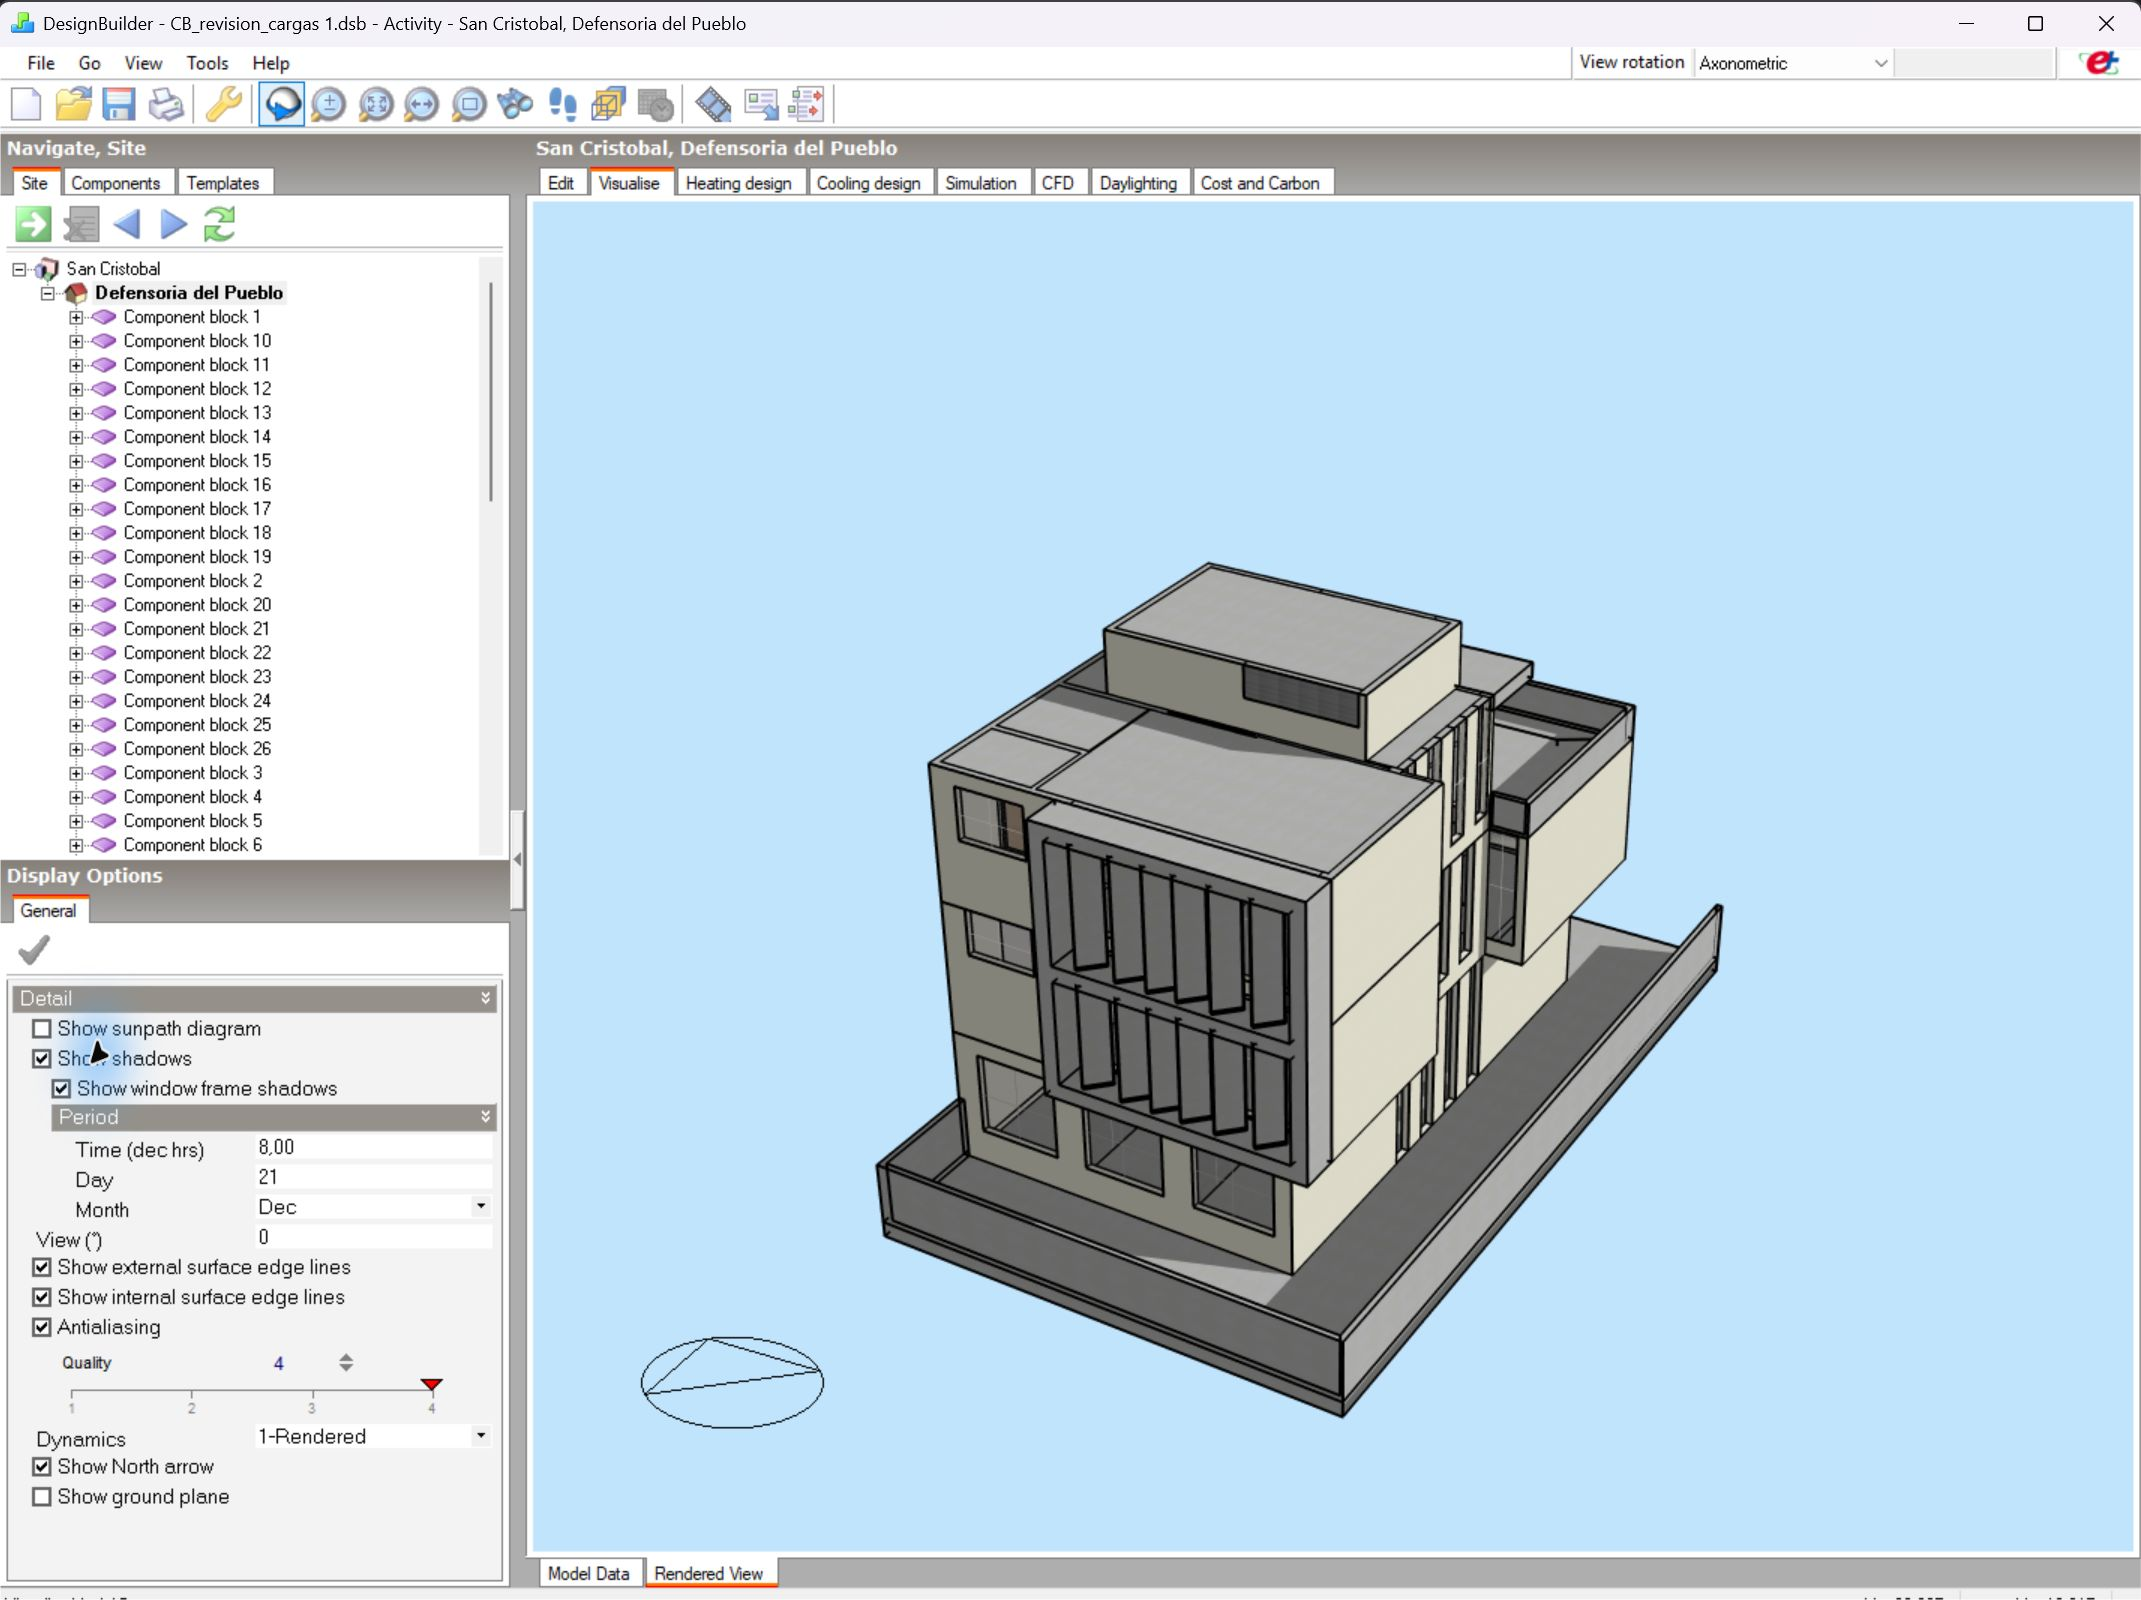
\includegraphics[trim=450bp 90bp 200bp 250bp,clip,width=0.95\textwidth,height=0.43\textheight,keepaspectratio]{figuras/db-modelo-atriocubierto.png}
\caption{Modelo energético con el atrio cubierto y las protecciones solares}
\label{fig:db-atrio-actual}
\fuente{Elaboración propia a partir de la vista del modelo revisado en DesignBuilder.}
\end{figure}

\clearpage
\subsection{Representación térmica del atrio}
\begin{textoDosTercios}
El atrio se divide en tres zonas de aire: primera planta alta, segunda planta alta y volumen superior. Esta división permite conservar las cotas y las relaciones con los recintos adyacentes. Las aberturas horizontales entre niveles se incluyen en la red de aire, mientras que la cubierta superior y la franja de cierre actúan como superficies térmicas opacas. El modelo no asigna ocupantes, iluminación, equipos ni climatización a las zonas del atrio.

Las rejillas se representan mediante componentes de biblioteca con coeficiente de descarga de 0,5 y disponibilidad permanente. Este coeficiente es un supuesto de modelación que debe contrastarse con el área libre y la ficha del producto seleccionado. La disponibilidad de las aberturas no constituye una medición de caudal ni demuestra, por sí sola, que la ventilación sea suficiente.
\end{textoDosTercios}

\begin{table}[H]
\centering
\caption{Condiciones de modelación del atrio cubierto}
\label{tab:db-atrio}
{\small\renewcommand{\arraystretch}{1.15}
\begin{tabular}{p{4cm}p{9cm}}
\toprule
Elemento & Representación en el modelo \\
\midrule
Base del atrio & Losa opaca sobre planta baja; se elimina el vidrio ficticio. \\
Continuidad vertical & Tres zonas conectadas por aberturas horizontales. \\
Conexión con pasillos & Pasos abiertos conservados en la red de aire. \\
Cierre superior & Cubierta opaca y franja adicional de $3,84\,\mathrm{m^2}$. \\
Ventilación exterior & Dos rejillas superiores; disponibilidad constante. \\
Coeficiente de descarga & 0,5, correspondiente al componente de biblioteca. \\
Cargas internas y HVAC & Sin ocupación, iluminación, equipos ni climatización. \\
\bottomrule
\end{tabular}}
\fuente{Elaboración propia a partir del modelo y de la comprobación del IDF exportado.}
\end{table}

\clearpage
\section{Construcción del modelo energético}
\subsection{Archivo climático y parámetros de cálculo}
\begin{textoDosTercios}
La simulación anual utiliza el EPW TMYx 2011--2025 de San Cristóbal. Se adopta el calendario 2025, desde el 1 de enero hasta el 31 de diciembre, para organizar los horarios de uso; esto no convierte el año meteorológico típico en un registro observado exclusivamente en 2025. La referencia horaria es UTC$-6$, sin horario de verano.

El cálculo de sombras utiliza el método por píxeles y las ventanas se representan individualmente. Esta configuración evita el límite de superposición de polígonos detectado con las protecciones solares y permite evaluar cada abertura sin multiplicadores de agrupación. La revisión conserva la geometría del atrio y los cerramientos del edificio.
\end{textoDosTercios}
\begin{table}[H]
\centering
\caption{Configuración de la simulación anual revisada}
\label{tab:db-configuracion}
{\small\renewcommand{\arraystretch}{1.12}
\begin{tabular}{p{4.2cm}p{8.8cm}}
\toprule
Parámetro & Valor o condición \\
\midrule
Motor de cálculo & EnergyPlus 9.4.0.002 \\
Archivo meteorológico & San Cristóbal, TMYx 2011--2025 \\
Periodo y calendario & 1 de enero--31 de diciembre de 2025 \\
Zona horaria & UTC$-6$; sin horario de verano \\
Paso de cálculo & 6 pasos por hora: 10 minutos \\
Zonas térmicas & 28 \\
Aberturas detalladas & 106 \\
Cálculo de sombras & Método por píxeles; ventanas sin agrupación \\
Climatización & Cargas ideales; consumo eléctrico no equivalente \\
Salón de usos múltiples & Actividad de 120 W/persona; factor metabólico 1 \\
\bottomrule
\end{tabular}}
\fuente{Elaboración propia a partir del IDF de la revisión del 12 de septiembre de 2026.}
\end{table}


\clearpage
\subsection{Visualización de las protecciones solares}
\begin{textoDosTercios}
La vista solar permite reconocer la relación geométrica entre cubiertas, celosías y fachadas. Se presenta como comprobación visual del modelo; no sustituye los balances anuales de radiación ni permite cuantificar ahorros energéticos. Las sombras mostradas corresponden al 21 de diciembre a las 08:00, según la configuración de visualización de DesignBuilder.
\end{textoDosTercios}
\begin{figure}[H]
\centering
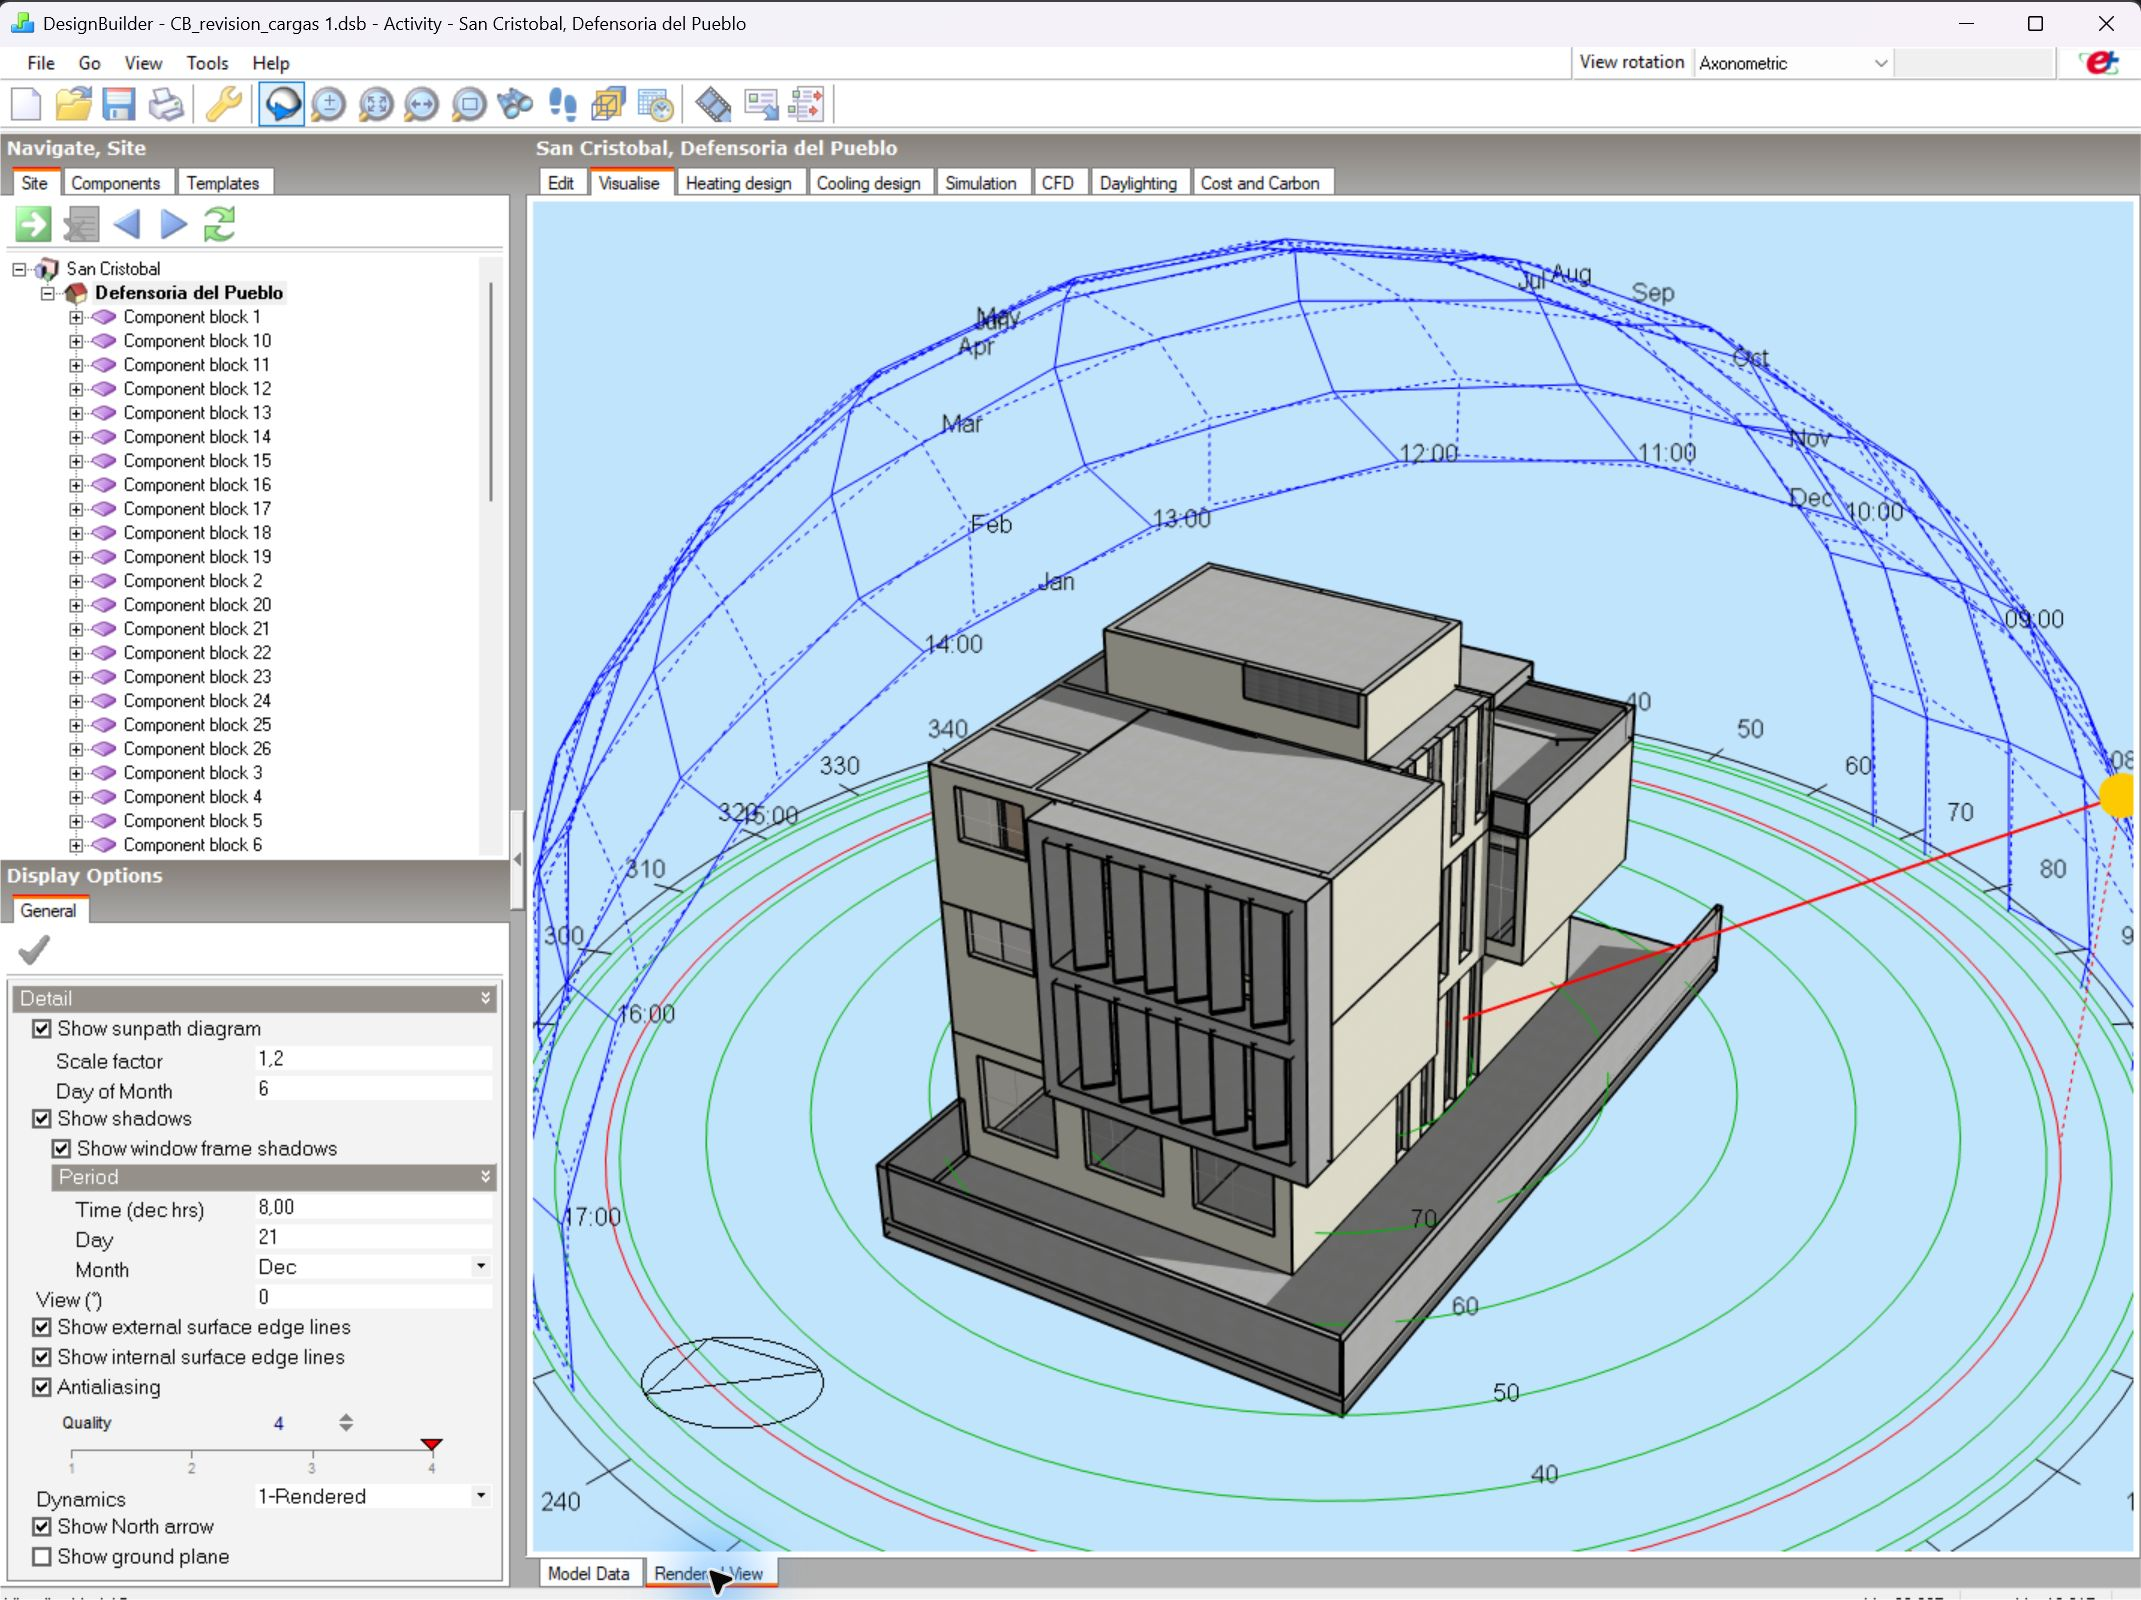
\includegraphics[trim=530bp 65bp 4bp 200bp,clip,width=\textwidth,height=0.55\textheight,keepaspectratio]{figuras/db-trayectoria-solar.png}
\caption{Vista solar del modelo con sus protecciones exteriores}
\label{fig:db-solar-actual}
\fuente{Elaboración propia mediante la visualización solar de DesignBuilder.}
\end{figure}


\clearpage
\subsection{Inventario de zonas y cargas internas}
\begin{textoDosTercios}
La tabla siguiente presenta las áreas y volúmenes explícitamente introducidos en el IDF. Estos valores corresponden a la geometría interior empleada en los balances y pueden diferir de las áreas calculadas sobre los polígonos de las superficies. Las áreas asignadas a niveles del atrio se conservan como parámetros de zona; no deben sumarse como superficie útil ocupable del edificio.
\end{textoDosTercios}
{\small\singlespacing
\setlength{\tabcolsep}{6pt}
\renewcommand{\arraystretch}{1.02}
\begin{longtable}{llrr}
\caption{Inventario geométrico de las zonas del modelo revisado}\label{tab:db-zonas}\\
\toprule
Nivel & Código de zona & Área IDF ($\mathrm{m^2}$) & Volumen ($\mathrm{m^3}$) \\
\midrule
\endfirsthead
\toprule
Nivel & Código de zona & Área IDF ($\mathrm{m^2}$) & Volumen ($\mathrm{m^3}$) \\
\midrule
\endhead
PB & PB-ES-01 & 5,36 & 18,48 \\
PB & PB-BO-01 & 2,08 & 7,17 \\
PB & PB-BA-01 & 4,58 & 15,81 \\
PB & PB-RE-01 & 9,33 & 32,18 \\
PB & PB-ASC & 2,57 & 8,86 \\
PB & PB-SE-01 & 54,10 & 186,64 \\
PB & PB-OF-03 & 13,46 & 46,45 \\
PB & PB-OF-02 & 9,87 & 34,07 \\
PB & PB-OF-01 & 12,72 & 43,87 \\
1PA & 1PA-DC & 7,85 & 23,60 \\
1PA & 1PA-ES & 9,12 & 27,30 \\
1PA & 1PA-ASC & 0,00 & 6,76 \\
1PA & 1PA-SR & 12,69 & 38,17 \\
1PA & 1PA-PAS & 21,85 & 65,69 \\
1PA & 1PA-OF-02 & 10,53 & 31,66 \\
1PA & 1PA-BA-02 & 4,85 & 14,58 \\
1PA & 1PA-BA-01 & 3,99 & 11,99 \\
1PA & ATRIO1PA & 14,57 & 43,81 \\
1PA & 1PA-OF-03 & 18,66 & 47,91 \\
1PA & 1PA-OF-01 & 15,20 & 45,69 \\
2PA & 2PA-BA-01 & 4,36 & 13,10 \\
2PA & 2PA-CAF & 5,85 & 17,59 \\
2PA & 2PA-ES & 8,85 & 26,43 \\
2PA & 2PA-SUM & 31,45 & 94,56 \\
2PA & 2PA-ASC & 2,26 & 6,74 \\
2PA & 2PA-PAS & 10,08 & 27,85 \\
2PA & ATRIO2PA & 0,00 & 42,38 \\
CUB & ATRIOSUPERIOR & 6,22 & 29,38 \\
\bottomrule
\end{longtable}
}
\fuente{Elaboración propia a partir de los campos explícitos de área y volumen de los 28 objetos Zone del IDF. Los vacíos del atrio no representan superficie útil ocupable.}

El área IDF nula del ascensor de primera planta y del atrio superior de segunda planta es un campo de entrada, no ausencia de volumen. EnergyPlus infiere 0,57 y 1,75 m\textsuperscript{2}, respectivamente, en el EIO. El hueco del atrio no constituye superficie útil de permanencia.


\clearpage
\subsection{Control de calidad y alcance de los resultados}
\begin{textoDosTercios}
La revisión distingue los errores que impiden ejecutar el cálculo de las advertencias que requieren una comprobación física. Se verificaron el cierre superior del atrio, sus conexiones de aire, la ausencia de cargas internas en el vacío y la eliminación de superficies auxiliares degeneradas. También se corrigió el factor metabólico del salón de usos múltiples: el valor 0,1 reducía la actividad seleccionada de 120 a $12\,\mathrm{W/persona}$. Se restableció el factor 1 sin modificar la densidad de ocupación.

La carga continua de $500\,\mathrm{W/m^2}$ del datacenter se conserva como dato pendiente de contraste. Las especificaciones describen un rack de 19UR, un switch de 48 puertos con consumo máximo aproximado de $49,3\,\mathrm{W}$ y un grabador de video previsto para operación continua \parencite[pp.~84--85, 101--102]{mogrovejoEspecificacionesElectricasGalapagos}. Estos antecedentes no acreditan por sí solos la potencia total introducida: se requiere el inventario definitivo de equipos.
\end{textoDosTercios}
\begin{table}[H]
\centering
\caption{Verificaciones y datos pendientes del modelo revisado}
\label{tab:db-verificacion}
{\small\singlespacing\renewcommand{\arraystretch}{1.10}
\begin{tabular}{p{3.7cm}p{9.3cm}}
\toprule
Comprobación & Estado y alcance \\
\midrule
Atrio cubierto & Cierre superior y pasos abiertos incorporados; cargas internas nulas. \\
Protecciones solares & Método por píxeles y ventanas individuales comprobados en el IDF. \\
Actividad del SUM & Corregida a 120 W/persona, conservando la densidad de ocupación. \\
Resolución temporal & Seis pasos por hora; contraste de estabilidad en la nueva corrida. \\
Cierre geométrico & Tres avisos se explican por subdivisiones de aristas; persisten encuentros de milímetros por revisar. \\
Red de aire & Dos aberturas horizontales utilizan una relación geométrica por defecto; requiere comprobar su representación. \\
Datacenter & 500 W/$\mathrm{m^2}$ continuos: pendiente del inventario de equipos. \\
Dimensionamiento & Confirmar calefacción y el día de diseño de invierno antes de validar capacidades. \\
\bottomrule
\end{tabular}}
\fuente{Elaboración propia a partir de la revisión del IDF y de los registros de EnergyPlus.}
\end{table}


\begin{textoDosTercios}
Los sistemas ideales calculan energía térmica, no consumo eléctrico. La comparación de escenarios requiere confirmar las cargas, los horarios y las eficiencias, además de resolver o justificar las incidencias que afectan los resultados.
\end{textoDosTercios}
